\documentclass[12pt]{article}
\usepackage{../template/NotesTeX}
\begin{document}
\setlength{\parskip}{\baselineskip}%
\graphicspath{ {/home/ab/school/notes/electeng101/} }

\title{Electeng101}
\author{Alexander Bailey}
\emailAdd{alexkingstonbailey@gmail.com}
\maketitle
\flushbottom

\section{Fundamentals of Electrical and Digital Systems}
\subsection{Electricity as Energy}
The fundamental concept that underpins the modern electrical `cycle' is: 
\begin{definition*}
  Energy is used to separate charges i.e the chemical reaction in a cell. This becomes the electric potential energy of the circuit
\end{definition*}

Separation of charge causes a difference in electric potential energy.
When this difference is applied to a closed circuit, charge will move around the circuit.
The movement of charge through is called a current. 

\subsubsection{Charge}
\begin{definition*}
  Electric charge is the physical property of matter that causes it to 

  experience a force when placed in an electromagnetic field. ($q$ or $Q$)
\end{definition*}

We (thanks to Benjamin Franklin) typically describe charge as having two states: postive (like a proton) and negative (like an electron).
These are not inherent to the universe but are just what we have defined.
Of course, the classic line is: `Like charges repel, opposite charges attract'.
Modeling the wire as a pipe carrying water, charge would be the amount of water. 

We model the strength of the electrostatic force as proportional to the charge of both particles and inversely proportional to the radius squared.
This is known as Coulomb's Law.

\begin{equation*}
  F \propto \frac{q_1q_2}{r^2}
\end{equation*}

Charge is measured in Coulombs (symbol C).
1C is is equivalent to approximately $6.3 \times 10^{18}$ electrons.

\subsubsection{Current}
\begin{definition*}
   Current is the rate of flow of charge represented by $i$ or $I$.
\end{definition*}

\marginnote{
  $I = {q\over t}$ \\
  or \\
  $I = \frac{dq}{dt}$
}[-1.1cm]

Current is defined numerically as the number of charges flowing through a particular point in one second.
Mathematically, it is the derivative of the total number of charges $q$ passing through a given section over time $t$ (written as $\frac{dq}{dt}$).
Current thusly has units of Coulombs per second ($\unit{Cs}^{-1}$) but Electrical Engineers have given this another name, the \textit{Ampere} (A).

\marginnote{Ampere also gave us the name current!}

Current gives Electrical Engineers an idea of how \textit{fast} energy is being used instead of how \textit{much} energy it has received\mn{Note that most electrical devices require a continuous supply of energy to function so speed is generally much more useful than amount }.
In the water analogy, current would be the speed of the water in the pipe. 

\begin{theorem*}
  \textbf{Conventional Current}

  Benjamin Franklin believed that electrical current was carried by positive charge `carriers', this led to \textit{centuries} of engineers using the wrong direction for current...
  Now we still use conventional current. BUT, electron flow is still in the other direction.
  Because of relative motion, a movement of negative charge in one direction is the \textbf{same thing} as a movement of positive charge in the other direction.
  Hence, it does not matter (for most things).
\end{theorem*}

\begin{theorem*}
  \textbf{Double-subscript notation}
  
  This notation indicates the directions charges are flowing in the order of \textbf{from} and \textbf{to}. 
  \begin{equation*}
    I_{ab} 
  \end{equation*}
  $I_{ab}$ is the current flowing from a to b.
\end{theorem*}

\begin{example}
  \begin{gather*}
    i = 0.5\unit{A } 
    t = 8\unit{min} = 60 \times 8 \unit{seconds} = 480\unit{seconds} \\
    i = \frac{dq}{dt} \\
    \implies q = \int_0^{480}0.5dt = [0.5t]_0^{480} \\
    \therefore q = 240\unit{C}
  \end{gather*}
\end{example}

\subsubsection{Voltage}
\begin{definition*}
  Voltage is the difference in electrical potential energy of each unit of charge between two points represented by $v$ or $V$.
\end{definition*}

Because a voltage is a difference, we must know what point in the circuit that the difference is measured relative to for it to make sense.
Voltage is commonly called a potential difference (PD) and has units Joules per Coulomb ($\unit{JC}^{-1}$).
Physically, it is the amount of energy lost or gained between two points. 
Using our water analogy, voltage would be the pressure of the water in the pipe.

Alessandro Volta decided that Joules per Coulomb ($\unit{JC}^{-1}$) was too difficult and gave us the \textit{Volt} (symbol V).
Additionally, every voltage must be accompanied by a \textit{voltage arrow}. 
This removes the ambiguity in which direction voltage is measured. 
The voltage arrow points in the direction of a \textit{potential rise}.

The voltage at A, with respect to B, is $V_{AB}$. 

\begin{theorem*}
  \textbf{Common Reference or Ground}

  Voltages are always measured between two points.
  It is convenient to define a reference where we can talk about voltages `at' a component.
  The location of ground is arbitrary and does not affect the actual voltages in the circuit.
  The `triangle' ground is for digital circuits while the `line' ground is for analog circuits.
\end{theorem*}
\begin{marginfigure}
  \vspace{ -1.8cm }
  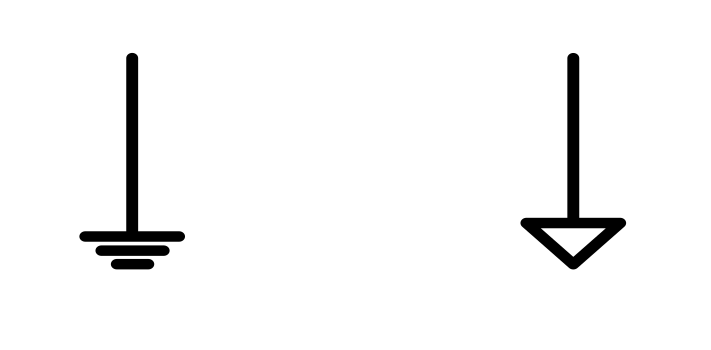
\includegraphics[scale=0.2]{grounds}
\end{marginfigure}


\begin{example}
  \begin{gather*}
    v = 2 - 6 \\
    v = iR \\
    -4 = 2i \\
    i = -2
  \end{gather*}
\end{example}
\begin{marginfigure}
  \vspace{ -1.5cm }
  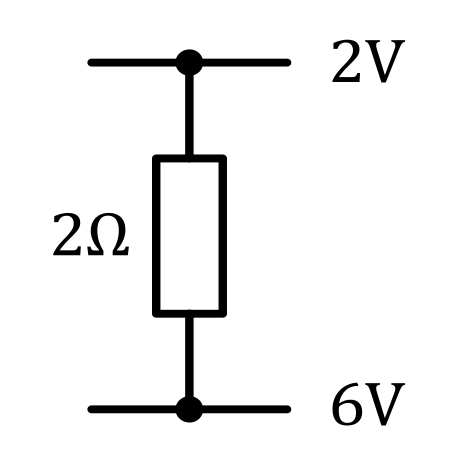
\includegraphics[scale=0.2]{example3}
\end{marginfigure}

\subsubsection{Resistance}

When electrical charge flows through a material, it must lose energy as it repels and collides with other charges.
The amount of energy lost depends on how `difficult' it is for the charge to flow. 
This difficulty depends on many factors including: stability of valence electrons, temperature, length and area.
These properties are summarised by \textit{resistance}.

\begin{equation*}
  v = i \times R 
\end{equation*}

From Ohm's Law, the amount of energy lost by the charges through a resistor is proportional to the rate at which charges slow through it.
The constant of proportionality $R$ from Ohm's Law is known as resistance. 
From this law, we can see resistance has units of Resistance has $\frac{V}{A}$.
We call this Ohms and give it the symbol Omega $(\Omega)$.

\begin{definition*}
  \textbf{The Passive-Sign Convention}

  When using Ohm's law there is an implicit sign convention that cannot be described by just the positive and negative symbols.
  A current is taken to be in the direction of a voltage drop. 
  This makes sense because charges can only lose energy through a resistor.
\end{definition*}

\subsection{Circuit Definitions}
Here are some conventions used to describe all circuits:

\begin{tabular}{c|c}
load & `destination' of the electricity i.e. a lightbulb \\
topology & the nature of the connections between components \\
nodes & the point where two or more components meet \\
\end{tabular}

When we are discussing values in a circuit, voltage is `across' a component, current is `through'. 
This means the voltage through a branch but we could also talk about the voltage `at' a component.
`at' means the PD is measured from the point to ground.

\begin{theorem*}
{\bf Circuit Topologies}
\begin{center}
\textbf{Closed}
\end{center}
The circuit has both flow of charge and energy transfer.

\begin{center}
\textbf{Open}
\end{center}

No electric potential means no flow of charge and no energy transfer. 
The circuit could be disrupted, i.e there is an air gap with (theoretically) infinite resistance.

\begin{center}
\textbf{Short}
\end{center}

The circuit (or circuit section) has a 0v potential difference.
This could mean a path of lower resistance meant no voltage `went' down that path or that voltages cancelled etc.
\end{theorem*}

\subsection{Components}

\subsubsection{Ideal Wire}
Ideal Wire has a resistance of 0$\Omega$. 
This means that no energy is lost when a current goes through it. 

\subsubsection{Voltage and Current Sources}
These sources can receive or output an \textit{infinite} amount of energy without deviating from their specification.
These are good models in most well-designed engineering applications because the sources are designed to operate within their limits.

Ideal Voltage Sources maintain a constant voltage across its terminals.
This means it will draw (or supply) whatever current is necessary to maintain that voltage.
Don't connect them in parallel.

Current sources don't actually exist.
But they maintain a constant current through its terminals regardless of voltage. 
This behaviour means that the voltage across it depends on the topology of the circuit.




\subsection{Models}
In Electrical Engineering (EE), a model is a description that communicates

\begin{itemize}
  \item Physical Characteristics 
  \item Electrical Function
  \item Magnitude
\end{itemize}

\marginnote{
Some EE models include:

\begin{itemize}
  \item Component Symbols 
  \item Schematics
  \item Block Diagrams 
  \item PCB Layouts 
\end{itemize}
}[-1cm]

\vspace{3pt}
Models allow you to more easily handle complex systems.
They compartmentalise systems into smaller sub-systems.
In circuit diagrams, component symbols are models of the actual components.
We can then focus on our actual engineering instead of {\it why} we are doing what we are doing (leave that to the physicists).

Mathematical Models, such as Ohm's Law, are still models. 
They simplify our calculations by making an approximation.

\section{SMART Engineering}
\begin{definition*}
  Systems of Monitoring, Analysis, and Response Technologies
\end{definition*}

\section{Electricity Supply}

\end{document}
